\subsection{Обучение метрики}

\begin{frame}{Сиамские сети, обучения по парам}
\centering
\begin{tabular}{m{15em} m{10em}}
    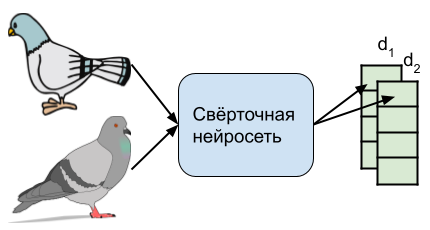
\includegraphics[width=0.38\textwidth]{images/siamse pigeon1.png} & 
    $
    \min_{d_1,\,d_2} \left( 1 - \frac{ d_1^\Tr d_2 }{\|d_1\|_2 \|d_2\|_2} \right)
    $
    \\
    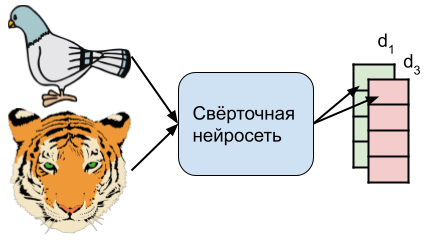
\includegraphics[width=0.38\textwidth]{images/siamse pigeon2.png} & 
    $
    \max_{d_1,\,d_3} \left( 1 - \frac{ d_1^\Tr d_3 }{\|d_1\|_2 \|d_3\|_2} \right)
    $
    \\
\end{tabular}

Если передавать метку $1$ для положительных пар и $-1$ для отрицательных, функцию ошибки можно записать в общем виде: $y_{ij} \left( 1 - \frac{ d_i^\Tr d_j }{\|d_i\|_2 \|d_j\|_2} \right) \rightarrow \min_{d_1,\,d_2}$

\end{frame}

\begin{frame}{Триплеты, схемы семплирования}

\begin{tabular}{m{14em} m{15em}}
    
\includegraphics[width=0.4\textwidth]{images/pigeon triplet1.png} &  
    --- случайное семплирование \\
    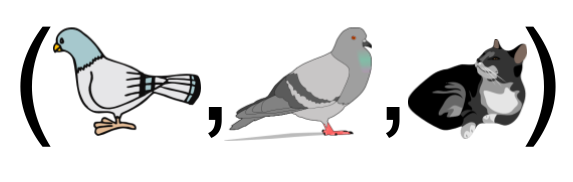
\includegraphics[width=0.4\textwidth]{images/pigeon triplet2.png} &  
    --- semi-hard negative sampling \\
    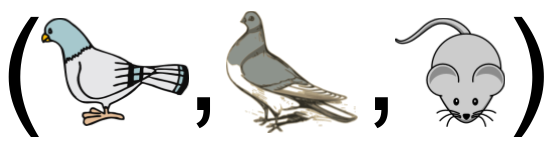
\includegraphics[width=0.4\textwidth]{images/pigeon triplet3.png} &  
    --- hard negative sampling, hard positive sampling
\end{tabular}

Мы хотим, чтобы расстояние от якорного примера до положительного было меньше, чем до отрицательного.

Hinge loss: $ [ m + dist(d_A, d_P) - dist(d_A, d_N) ]_+ $
    
\end{frame}

\begin{frame}{Ещё обучения метрики}

\begin{itemize}
    \item Можно добавить пару к негативному примеру, получим квадруплеты!
    \item Можно пользоваться особенностью обучения по батчам, и семплировать примеры только изнутри батча.
    \item Используя матричные формы функции ошибки можно без семплирования оптимизировать сразу по всем возможным парам из батча.
    \item Можно формировывать псевдо-классы. И вместо отсемплированных примеров, брать эти псевдоклассы (Proxy-NCA).
    \item И ещё много идей...
\end{itemize}
    
\end{frame}

\begin{frame}{Но в реальности...}

Так всё это обучение метрик вообще помогает?

\begin{center}
    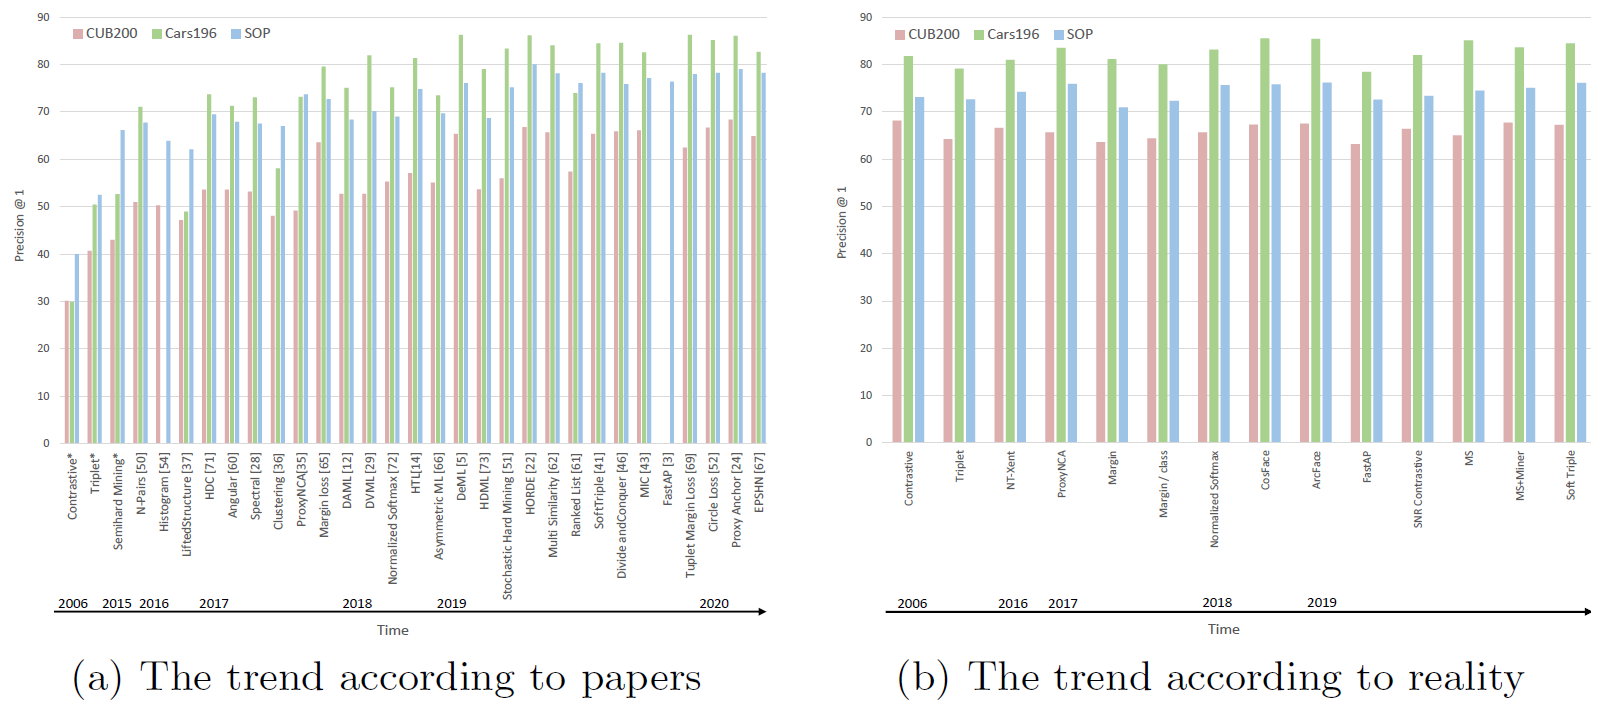
\includegraphics[width=0.9\textwidth]{images/reality check.png}
\end{center}
\end{frame}
